\documentclass{article}

%----------------------------------------
% Packages
%----------------------------------------
\usepackage[left=1in, right=1in, top=1in, bottom=1in]{geometry}
\usepackage{graphicx}
\usepackage{amsmath,amsbsy,amssymb,amsfonts,amsthm}
\usepackage{nicefrac}
\usepackage{mathtools}
\usepackage{color}
\usepackage{xspace} % Correct macro spacing
\usepackage[numbers]{natbib} % For citations
\usepackage{times}
\usepackage{graphicx,subfigure}
%\usepackage[small,bf]{caption}
\usepackage{algorithm,algorithmic} 
\usepackage{hyperref}
\usepackage{graphbox}

\usepackage{xcolor}
\usepackage{shadethm}

\usepackage{fancyhdr}
\pagestyle{fancy}
\lhead{This is my name}
\rhead{this is page \thepage}

\usepackage{fancyhdr}
\pagestyle{fancy}
\lhead{IFT 6085 - Theoretical principles for deep learning}
\rhead{Lecture 2: January 9, 2020}


\newshadetheorem{thm}{Theorem}
\newshadetheorem{lemma}{Lemma}
\newshadetheorem{defn}{Definition}
\newshadetheorem{assm}{Assumption}
\newshadetheorem{prop}{Property}
\newshadetheorem{eg}{Example}

\usepackage{amsmath}

\DeclareMathOperator*{\argmax}{\arg\max}
\DeclareMathOperator*{\argmin}{\arg\min}
\DeclareMathOperator*{\E}{\mathbb{E}}
\DeclareMathOperator*{\I}{\mathbb{I}}
\DeclareMathOperator*{\V}{\mathbb{V}}

\newcommand{\diag}[0]{\operatorname{diag}}
\newcommand{\vect}[1]{\mathbf{#1}}
\newcommand{\vects}[1]{\boldsymbol{#1}}
\newcommand{\matr}[1]{\mathbf{#1}}
\newcommand{\matrs}[1]{\boldsymbol{#1}}

\renewcommand{\P}[0]{\mathbb{P}}
\newcommand{\Q}[0]{\mathbb{Q}}

\DeclareMathOperator*{\tr}{tr}
\DeclareMathOperator*{\prox}{prox}
\DeclareMathOperator*{\conv}{conv}
\DeclareMathOperator*{\dom}{dom}
\DeclareMathOperator*{\minimize}{minimize}
\DeclareMathOperator*{\maximize}{maximize}
\DeclareMathOperator*{\sign}{sign}
\DeclareMathOperator*{\vecop}{vec}
\DeclareMathOperator*{\Poisson}{Poisson}
\DeclareMathOperator*{\Cat}{Cat}
\DeclareMathOperator*{\Dir}{Dir}
\DeclareMathOperator*{\Exp}{Exp}
\DeclareMathOperator*{\DiscreteUniform}{DiscreteUniform}
\DeclareMathOperator*{\Uniform}{Uniform}
\newcommand{\R}{\mathbb{R}}
\newcommand{\N}{\mathbb{N}}
\newcommand{\X}{\mathcal{X}}

\DeclarePairedDelimiter{\abs}{\lvert}{\rvert}
\DeclarePairedDelimiter{\norm}{\lVert}{\rVert}
\DeclarePairedDelimiter{\inprod}{\langle}{\rangle}
\DeclarePairedDelimiter{\biginprod}{\big\langle}{\big\rangle}
\DeclarePairedDelimiter{\Biginprod}{\Big\langle}{\Big\rangle}
\DeclarePairedDelimiter{\bigginprod}{\bigg\langle}{\bigg\rangle}
\DeclarePairedDelimiter{\Bigginprod}{\Bigg\langle}{\Bigg\rangle}
\DeclarePairedDelimiter{\floor}{\lfloor}{\rfloor}


\definecolor{shadethmcolor}{HTML}{F0F0F0}
%\definecolor{shadethmcolor}{HTML}{EDEDED}
%\definecolor{shadethmcolor}{HTML}{EDF8FF}
%\definecolor{shaderulecolor}{HTML}{EDF8FF}
%\definecolor{shaderulecolor}{HTML}{45CFFF}
\setlength{\shadeboxrule}{.4pt}


\setlength\parindent{0pt}

% Packages hyperref and algorithmic misbehave sometimes.  We can fix
% this with the following command.
\newcommand{\theHalgorithm}{\arabic{algorithm}}

%----------------------------------------
% Standard macros
%----------------------------------------


%----------------------------------------
% Project-specific macros
%----------------------------------------

%----------------------------------------
% Header
%----------------------------------------
\title{IFT 6085 - Lecture 2 \\ 
Basics of convex analysis and gradient descent }
\date{}

%----------------------------------------
% Document
%----------------------------------------
\begin{document} 

%----------------------------------------
% Abstract
%----------------------------------------
\maketitle


\textbf{Scribes}\hfill
\textbf{Instructor:}  Ioannis Mitliagkas\\
\textbf{Winter 2020:} Joss Rakotobe\\
\textbf{Winter 2019:} Andrew Williams, Ankit Vani, Maximilien Le Clei\\
\textbf{Winter 2018:} Assya Trofimov, Mohammad Pezeshki, Reyhane Askari


%----------------------------------------
% Body
%----------------------------------------

\newcommand{\infgc}{\inf_{g \in \mathcal{C}}}
\newcommand{\supgc}{\sup_{g \in \mathcal{C}}}


\section{Introduction}
 
Many machine learning problems involve learning parameters $\theta \in \Theta$ of a function $f$ towards achieving an objective better. Typically, such objectives are characterized by a loss function $L: \Theta\to\R$, also called the empirical risk, and training the model corresponds to searching the optimal parameters $\theta^\ast$ that minimize this loss.\\

For example, in supervised learning, $\theta$ parameterizes a function $f: X\to Y$, where any $x \in X$ is an input and any $y \in Y$ is a target label. Then,
\[
L(\theta) = \frac{1}{n}\sum_{i=1}^n \ell(f(x_i; \theta), y_i)
\]
represents the loss function for a dataset containing $n$ training examples $(x_1,y_1),\ldots,(x_n,y_n)$. Here, $\ell$ is a deterministic function that determines the distance between a target label $y_i$ and the predicted label $y_i' = f(x_i; \theta)$. In this setting, learning is carried out by performing \emph{empirical risk minimization}, which involves optimizing to find parameters $\theta^\ast \in \argmin_{\theta\in\Theta} L(\theta)$.\\

In the first few lectures, we will dive deeper into the basics and theory of optimization that lie at the heart of machine learning. We will step back from the notation we see in machine learning, and start by considering the most general unconstrained optimization problem\footnote{More generally, this would involve an $\inf$ instead of $\min$, but in this lecture we keep the notation simple and stick with $\min$.} for a real valued function $f:\X\to\R$:
\[
\min_{x\in\X} f(x)
\]
In most of our discussions, we will consider $\X$ or $\dom(f)$ to be the $d$-dimensional Euclidean space $\R^d$.\\

The optimization problem formulated above is NP-hard in general (see \cite{bubeck2015convex}. Section 6.6). However, for certain classes of functions $f$, strong theoretical guarantees and efficient optimization algorithms exist. In this lecture, we consider such a class of functions, called \emph{convex functions} and prove convergence guarantees for an algorithm for convex optimization called \emph{gradient descent}.


\section{Convex optimization}

    This section introduces some concepts in convexity, and then uses them to prove convergence of gradient descent for convex functions.\\
    
    Although in practice people commonly use the same algorithms for non-convex optimization as they do for convex optimization (e.g.\ gradient descent), it is important to note that the strong theory for convex optimization algorithms often breaks down without the convexity assumption.
    However, ideas from convex analysis and the weakening of certain results can give partial guarantees and offer generalizations for non-convex analysis.


\subsection{Background}

\subsubsection{Lipschitz continuity}

\begin{defn}[Lipschitz continuity]
Let $L\geq 0$. A real-valued function $f$ is $L$-Lipschitz continuous iff $\forall x,y \in \dom f$,
\[
	\abs{f(x) - f(y)} \leq L\norm{x-y}
\]
\end{defn}

Intuitively, a Lipschitz continuous function is bounded in how fast it can change. Figure~\ref{fig:lipschitz} illustrates two Lipschitz continuous functions with different Lipschitz constants.

\begin{figure}[ht]
\centering
    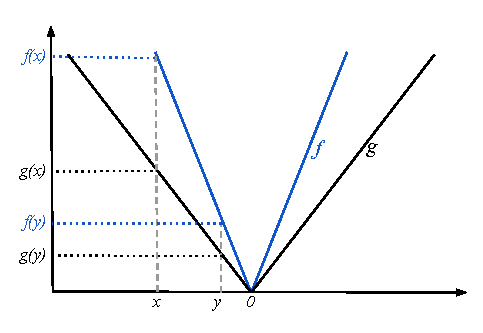
\includegraphics[width=0.4\textwidth]{figures/Lipschitz.pdf}
    \caption{Consider a $L_f$-Lipschitz continuous function $f$ and a $L_g$-Lipschitz continuous function $g$. If $f$ and $g$ are changing as fast as they can, then $L_f > L_g$.}
    \label{fig:lipschitz}
\end{figure}

% ------ Max --------
% In this example, |f(x) - f(y)| > |g(x) - g(y)| meaning that the smallest value L_f can take is higher than the smallest value L_g can take. 
% -------------------

As another example, consider the following function:
\[
    f(x)= 
\begin{cases}
    \exp(-\lambda x),& \text{if } x > 0\\
    1,              & \text{otherwise}
\end{cases}
\]
$f(x)$ here is $L$-Lipschitz, and the value of $L$ increases with $\lambda$.
As the value of $\lambda$ increases, the function gets closer to discontinuity.
In the limit of $\lambda$ going to $\infty$, we recover a step function, which is not Lipschitz continuous for any $L$.
In fact it is not continuous at $x=0$.
This function is illustrated in Figure~\ref{fig:lambda}.

\begin{figure}[ht]
\centering
    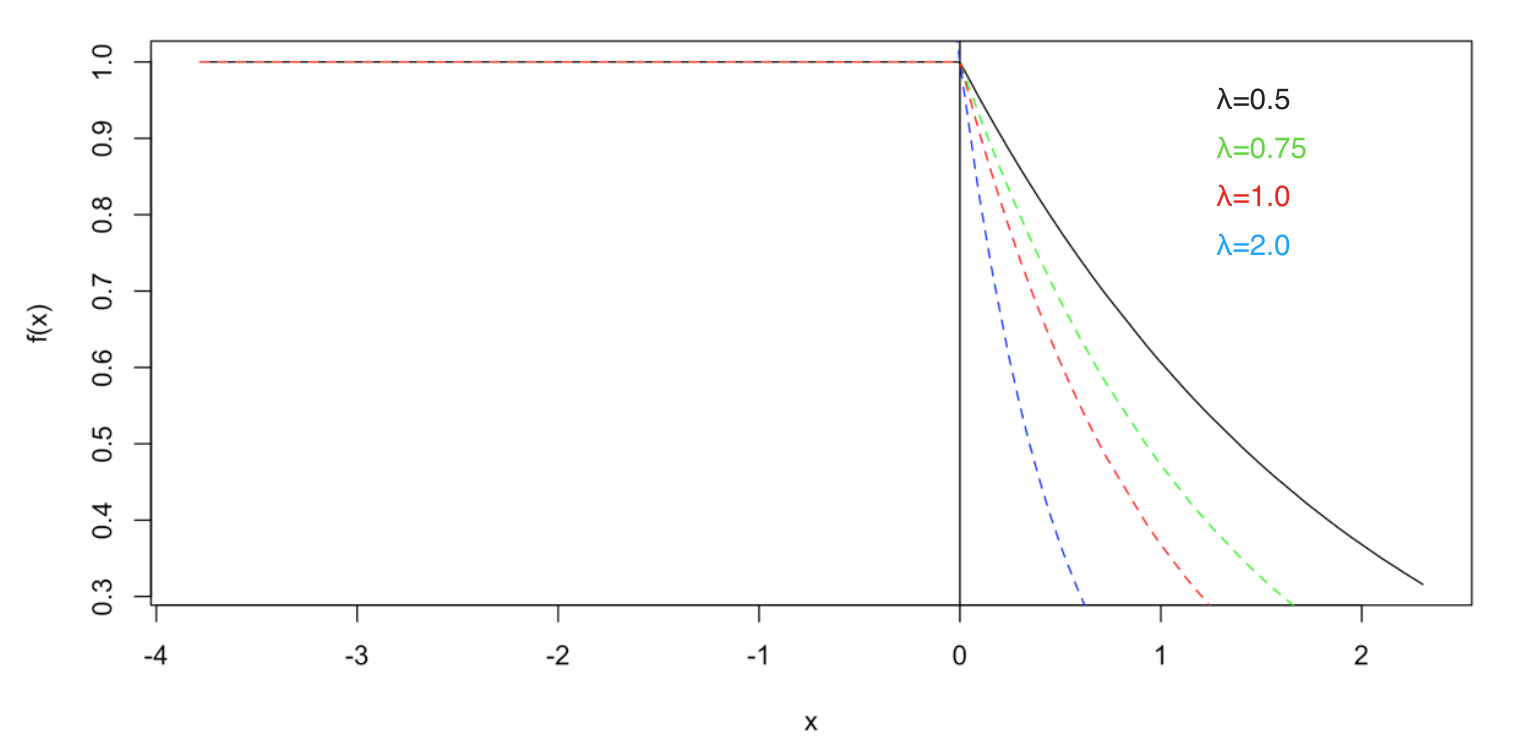
\includegraphics[width=0.7\textwidth]{lambda.png}
    \vspace{-10px}
    \caption{As $\lambda$ increases in $f(x)$, the Lipschitz constant $L$ increases, and the function gets closer to being discontinuous.}
    \label{fig:lambda}
\end{figure}

A Lipschitz continuous function does not need to be differentiable. For example, we can have integer-valued and non-smooth Lipschitz continuous functions. However, a corollary of $f$ being $L$-Lipschitz continuous is that if it is differentiable, the norm of its gradient is bounded by $L$.

\begin{lemma}[First order condition for Lipschitz continuity]\label{lemma:lip}
    A differentiable function $f$ is $L$-Lipschitz continuous iff the norm of its gradient is bounded by $L$:
    \[
    \forall x \in \dom(f), \norm{\nabla f(x)} \leq L
    \]
\end{lemma}{}

\begin{proof}
We first give the idea in $\R$, then generalize in $\R^d$.\\\\
$(\implies)$
For $\dom(f)\subseteq\R$,
\begin{align*}
	f'(x) &= \lim_{y\to x} \frac{f(x)-f(y)}{x-y} \tag{definition of derivative}\\
	\implies \abs{f'(x)} &= \lim_{y\to x} \frac{\abs{f(x)-f(y)}}{\abs{x-y}} \leq L \tag{definition of Lipschitz continuity}
\end{align*}

In general, if $\dom(f)\subseteq \R^d$ for a differentiable $L$-Lipschitz function $f$, then
\[
    \norm{\nabla f(x)} \leq L
\]
In fact, let $u\in\mathbb{S}^d$ a unit vector, then the directional derivative with respect to $u$ is given by:
\begin{align*}
	\nabla_u f(x) &= \lim_{h\to 0} \frac{f(x+hu)-f(x)}{h} \tag{definition of directional derivative}\\
	\implies \abs{\nabla_u f(x)} &= \lim_{h\to 0} \frac{\abs{f(x+hu)-f(x)}}{\norm{hu}} \leq L \tag{definition of Lipschitz continuity}
\end{align*}

Since  $\nabla_u f(x)=\langle\nabla f(x),u\rangle$, taking $u=\frac{\nabla f(x)}{\norm{\nabla f(x)}} \implies \nabla_u f(x)=\norm{\nabla f(x)}$, thus the result.\\


$(\impliedby)$ By contraposition, suppose there exist $A,B\in \dom(f)$ such that $|f(A)-f(B)|>L\norm{A-B}$.\\

In the multivariate case, the mean value theorem states that there exists a point C in the line segment $\overline{AB}$ such that $f(A)-f(B)= \langle\nabla f(C), A-B \rangle$.\\
Hence, by Cauchy-Schwarz inequality, $|f(A)-f(B)|\leq \norm{\nabla f(C)} \norm{A-B}$, which implies that $$\norm{\nabla f(C)}\geq \frac{|f(A)-f(B)|}{\norm{A-B}}> L$$.

\end{proof}{}

Note that Lipschitz continuity is a special case of continuity: all Lipschitz continuous functions are continuous, but not all continuous functions are Lipschitz continuous (for more information, see \cite{boyd2004convex}).



\subsubsection{Convex sets}

Before we define convex sets, let us first define a convex combination, which is a constrained version of a linear combination, illustrated in Figure~\ref{fig:two_points} for two points.

\begin{defn}[Convex combination]
If $z \in \R^d$ is a linear combination of $x_1, x_2,\ldots,x_n \in \R^d$ and the coefficients are non-negative and sum to $1$, then $z$ is a convex combination of $x_1, x_2,\ldots,x_n$:
\[
    z = \sum_{i=1}^n\theta_i x_i, \quad\text{ where } \forall i \in (1,\ldots,n), \theta_i \geq 0 \text{ and } \sum_{i=1}^n \theta_i = 1
\]
\end{defn}

\begin{figure}[ht]
\centering
    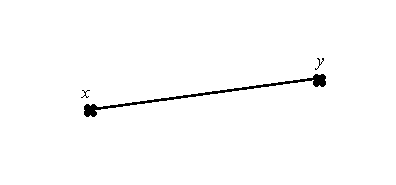
\includegraphics[width=0.3\textwidth]{figures/line_two_points.pdf}
    \caption{All convex combinations $z = \theta x + (1-\theta)y$ of two points $x$ and $y$ lie on the line segment from $x$ to $y$. When $\theta=1$, we get $x$ and when $\theta=0$, we get $y$.}
    \label{fig:two_points}
\end{figure}


\begin{defn}[Convex set]
$\X$ is a convex set if the convex combination any two points in $\X$ is also in $\X$. That is, for a convex set $\X$:
\[
\forall x,y \in \X, \forall \theta \in  [0, 1],\quad z = \theta x + (1-\theta)y \in \X
\]
\end{defn}

Figure~\ref{fig:sets} gives examples of a convex set and a non-convex set.

\begin{figure}[ht]
\centering
    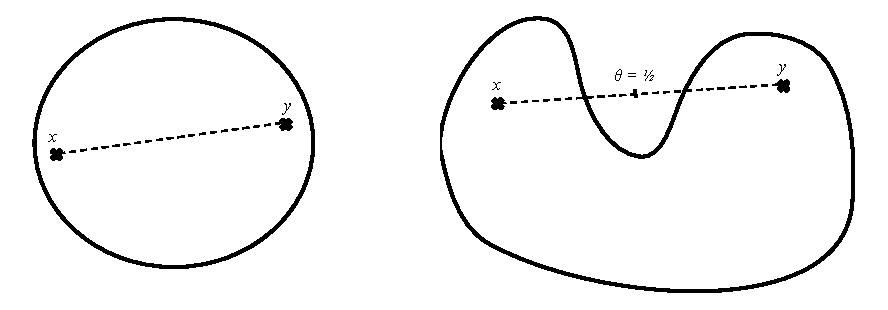
\includegraphics[width=0.6\textwidth]{figures/sets.pdf}%
    \caption{Examples of a convex and a non-convex set. \textbf{Left:} Convex set, \textbf{Right:} Non-convex set.}
    \label{fig:sets}
\end{figure}


\subsubsection{Convex functions}
Armed with the definition of convex sets,
we can finally define convex functions.

\begin{defn}[Convex function]
A function $f(x)$ is \emph{convex} iff the domain $\dom(f)$ is a convex set and $\forall x,y \in \dom(f), \forall \theta \in [0,1]$,
\[
	f(\theta x+ (1-\theta)y) \leq \theta f(x) + (1-\theta)f(y)
\]
\label{def:convex}
\end{defn}

The condition above says that for any two members in the domain of $f$, the function's value on a convex combination does not exceed the convex combination of those values. It can be viewed as a \textit{zeroth order condition}, as it doesn't involve any condition of differentiability of the function. We will see results with higher order conditions later.\\
Graphically, when $f$ is convex, for any points $x$ and $y$ in $f$'s domain, the chord connecting $f(x)$ and $f(y)$ lies above the function between those points. This is illustrated in Figure~\ref{fig:convex}.\\

For a convex function $f$, its opposite function $-f$ is defined as a \emph{concave} function. In other words, for a concave function, the inequality condition in Definition~\ref{def:convex} is reversed.\\

\begin{figure}[ht]
\centering
    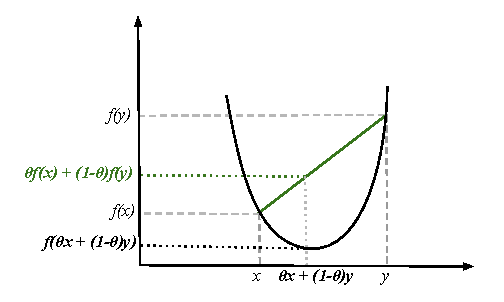
\includegraphics[height=0.2\textheight]{figures/convex.pdf}
    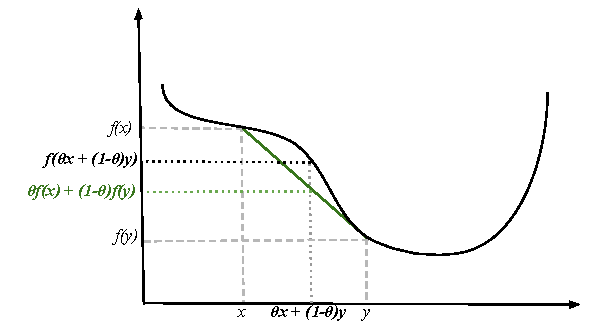
\includegraphics[height=0.2\textheight]{figures/quasi-convex.pdf}
    \caption[]{\textbf{Left:} Example of a convex function. For any two points $x,y \in \dom(f)$, the chord $\theta f(x) + (1-\theta)f(y), \theta \in [0,1]$ lies above the function value $f(\theta x+ (1-\theta)y), \theta \in [0,1]$. \textbf{Right:} Example of a non-convex function\footnotemark[2]. We see here that there exist points $x$ and $y$ for which the chord lies below the curve between $f(x)$ and $f(y)$.}
    \label{fig:convex}
\end{figure}
\footnotetext[2]{In fact, this is an example of a quasiconvex function $f$, meaning that all sublevel sets $S_\alpha(f)=\{x \mid f(x) \leq \alpha\}$ are convex sets.}

As we can see in Figure \ref{fig:convex}, convexity is not a necessary condition for a function to have a unique global minimum.
The right plot shows an example of non-convex function having a unique global minimum.


\subsection{First-order conditions for convexity}

We will see that for differentiable and twice differentiable functions, it is possible to define convexity in terms of first- and second-order conditions for convexity.
Note that all the definitions of convexity are equivalent when the appropriate level of differentiability holds (for more information, see \cite{bubeck2015convex}).

\begin{lemma}[First order condition for convexity]\label{lemma:first}
A differentiable function $f$ is convex iff $\dom(f)$ is convex and $\forall x, y \in \dom(f)$,
\[
	f(y) \geq f(x) + \nabla f(x)^\top(y-x)
\]
\end{lemma}

\begin{proof}
$(\implies)$ Suppose f is convex. By definition of a convex function, $\dom(f)$ is convex. Let $x,y\in\dom(f)$ and $\theta\in[0,1]$,

\begin{align*}
	&  &f((1-\theta)x+ \theta y) \quad &\leq \quad (1-\theta) f(x) + \theta f(y) \tag{definition of convexity}\\
	&\implies \quad &f(x+\theta (y-x)) \quad &\leq \quad f(x) + \theta (f(y)-f(x))\\
	&\implies \quad  &\frac{f(x+\theta (y-x)) - f(x)}{\theta} \quad &\leq \quad f(y)-f(x)\\
	&\implies \quad &\frac{f(x+\theta u) - f(x)}{\theta} \quad  &\leq \quad f(y)-f(x) \tag{$u=y-x$}\\
	&\implies \quad &\nabla_u f(x) \quad  &\leq \quad f(y)-f(x) \tag{taking $\theta\to 0$}
\end{align*}{}
Since $\nabla_u f(x)=\langle\nabla f(x),u\rangle=\nabla f(x) ^\top u=\nabla f(x)^\top (y-x)$, the result follows.\\

$(\impliedby)$
Suppose $\dom(f)$ is convex and
\[
\forall x, y \in \dom(f), f(y) \geq f(x) + \nabla f(x)^\top(y-x)
\]
Let $x,y\in\dom(f), \theta \in [0,1]$.\\

By the convexity of $\dom(f)$, $z=\theta x + (1-\theta)y \in \dom(f)$\\

Applying the above inequation using $z$: 
\begin{align}
    f(x) \geq f(z) + \nabla f(z)^\top(x-z) \label{eq1}\\
    f(y) \geq f(z) + \nabla f(z)^\top(y-z) \label{eq2}
\end{align}{}
Multiplying inequation (\ref{eq1}) by $\theta$, inequation (\ref{eq2}) by $1-\theta$ and adding, we get:

\begin{align*}
    \theta f(x) + (1-\theta) f(y) &\geq \theta(f(z) + \nabla f(z)^\top(x-z))+(1-\theta)(f(z) + \nabla f(z)^\top(y-z))\\
    &= \theta f(z)+ \nabla f(z)^\top (\theta x - \theta z) +  (1-\theta) f(z)+ \nabla f(z)^\top ((1-\theta) y - (1-\theta) z)\\
    &= f(z)+ \nabla f(z)^\top (\theta x + (1-\theta)y - z)\\
    &=f(z)\\
    &=f(\theta x + (1-\theta)y)
\end{align*}{}
    
\end{proof}{}

Intuitively, this says that for a convex function, a tangent of its graph at any point must lie below the graph. This is illustrated in Figure~\ref{fig:firstorder}.\\

\begin{figure}[ht]
\centering
    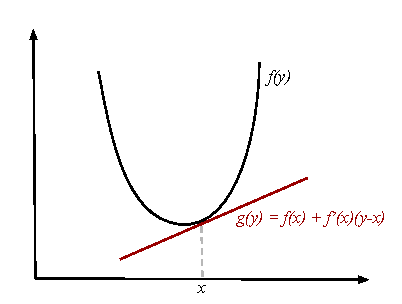
\includegraphics[height=0.2\textheight]{figures/first_order.pdf}
    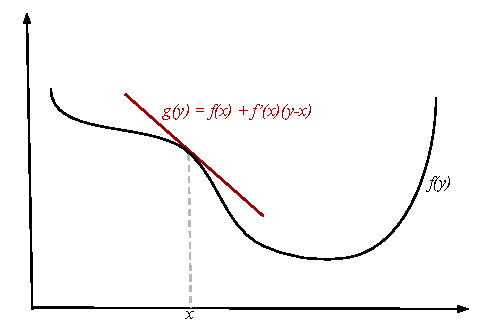
\includegraphics[height=0.2\textheight]{figures/first_order_quasi.pdf}
    \caption{Example of a convex and a non-convex function illustrating the first-order condition for convexity. For the convex function on the left, all possible tangents will lie below the graph. However, for the non-convex function on the right, there exists a tangent such that it lies above the graph for some points in the function's domain.}
    \label{fig:firstorder}
\end{figure}

\subsection{First- and second-order conditions for convexity}
Before discussing the second-order condition for convexity, let us review the multivariate generalization of a second derivative, namely a \emph{Hessian}:
\[
\nabla^2 f(x) = \begin{bmatrix}
\frac{\partial^2 f}{\partial x_1^2} & \frac{\partial^2 f}{\partial x_1 \partial x_2} & \ldots & \frac{\partial^2 f}{\partial x_1 \partial x_d}\\
\vdots & \vdots & \ddots & \vdots\\
\frac{\partial^2 f}{\partial x_d \partial x_1} & \frac{\partial^2 f}{\partial x_d \partial x_2} & \ldots & \frac{\partial^2 f}{\partial x_d^2}
\end{bmatrix}
\]
For a function $f:\R\to\R, f(x) = \frac{h}{2}x^{2}$, the second derivative $f''(x) = h$ corresponds to a measure on how quickly the slope of the function can change. Similarly, the Hessian represents the curvature of a function $f$ with $\dom(f)\subseteq \R^d$. A multivariate quadratic function $f$ can be written as $f(x) = \frac{1}{2}x^\top Hx $, where $H$ is the Hessian. The eigenvalues of the Hessian determine the curvature of the function along its eigenvectors. Consider the eigendecomposition\footnotemark[3]
\footnotetext[3]{The Schwarz Theorem implies that the Hessian is always a symmetric matrix. Applying the spectral theorem, it can always be decomposed in the mentioned form, with $Q$ an orthogonal matrix, i.e., $Q^{-1}=Q^T$.}
\begin{equation}\label{eigendec}
	H = Q\Lambda Q^\top
\end{equation}{}
where
\[
  \Lambda = \begin{bmatrix}
    \lambda_1 & & & \\
    & \lambda_2 & & \\
    & & \ddots & \\
    & & & \lambda_4 \\
  \end{bmatrix}
\]

Changing the basis to $Q$, we can focus on the directions described by $Q=[q_{1},q_{2},\ldots,q_{d}]$. Then, along the direction $q_{i}$, we get the curvature $\lambda_{i}$. Figure~\ref{fig:curvature2} illustrates the curvature of a convex quadratic function. Note that not every quadratic functions are convex (see Lemma \ref{second}).

\begin{figure}[ht]
\centering
    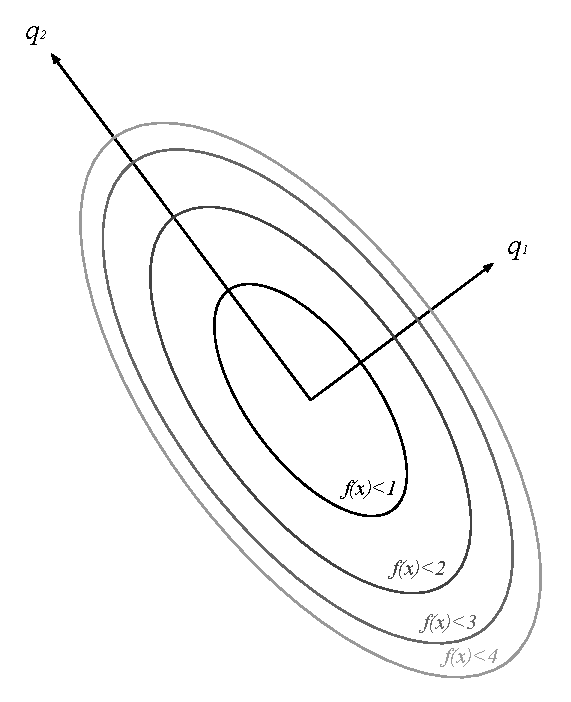
\includegraphics[align=c,width=0.33\textwidth]{figures/curvature2.pdf}\qquad\qquad
    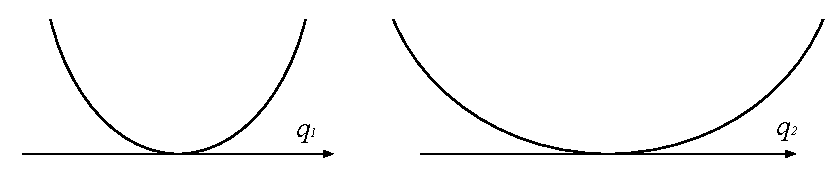
\includegraphics[align=c,width=0.45\textwidth]{figures/curvature.pdf}
    \caption[]{\textbf{Left:} Looking along the principle directions of the quadratic function $f(x) = \frac{1}{2}x^\top Hx $, we see that the curve changes faster along $q_1$ than $q_2$. Here\footnotemark[4], $\lambda_1 > \lambda_2$. \textbf{Right:} Cross-sections along $q_1$ and $q_2$, showing that $f$ has higher curvature along $q_1$ than $q_2$.}
        \label{fig:curvature2}
\end{figure}
\footnotetext[4]{Most eigendecomposition algorithms return eigenvalues in non-decreasing order.}

\begin{defn}[Positive semi-definite]
A symmetric matrix $M\in \R^{d\times d}$ is positive semi-definite if
\[
\forall x\in \R^d, x^\top M x \geq 0
\]
In that case, we will use the notation $M \succeq 0$.
\end{defn}{}

A positive semi-definite matrix does not necessarily have all positive elements \footnotemark[5]\footnotetext[5]{There exist matrices with all positive entries, that are not positive semi-definite, and there exist positive semi-definite matrices that have negative elements}. However, as we will see in the next theorem, its eigenvalues $\lambda_i$ are non-negative.\\

\begin{thm}[Characterization of a positive semi-definite matrix]
A symmetric matrix $M\in \R^{d\times d}$ is positive semi-definite iff all its eigenvalues $\lambda_i$ are non-negative: $\forall i \in \{1,\ldots,d\},$
\[
    \lambda_i \geq 0
\]
\end{thm}{}

\begin{proof}
Suppose $M\succeq 0$ and denote $v_i$ an eigenvector associated to $\lambda_i$. Then, using the definition of an eigenvalue and eigenvector, we have $\forall i \in \{1,\ldots,d\},$
\[
0 \leq v_i^\top M v_i = v_i^\top \lambda_i v_i =\lambda_i \norm{v_i}^2
\]
Hence, $\lambda_i\geq 0$.\\

Suppose $\lambda_i \geq 0$ for $i=1,\ldots,d$. Then, using the eigendecomposition of $M$, $M=Q \Lambda Q^\top$ as mentioned previously in equation (\ref{eigendec}), $\forall x \in \R^d$,
\[
    x^\top M x = x^\top Q \Lambda \underbrace{Q^\top x}_{y} = y^T \Lambda y = \sum_{i=1}^d \lambda_i y_i^2\geq 0
\]
\end{proof}

Before stating the second order condition for convexity, we will need a small but useful other lemma.

\begin{lemma}\label{line}
A function f is convex iff $\dom(f)$ is a convex set and $\forall x \in \dom(f), v\in\R$, the real function $g_{x,v}$ is convex, where
$$g_{x,v}(t):=f(x+tv)$$
for all $t\in \R$ such that $x+tv\in\dom(f)$.
\end{lemma}{}

\begin{proof}
$(\implies)$ Suppose $f$ is convex, then by definition of a convex function, $\dom(f)$ is a convex set.\\

First, we prove that $\dom(g_{x,v})$ is a convex set.\\

$\forall s,t\in \dom(g_{x,v}), \theta\in[0,1]$, we have $x+sv\in\dom(f)$ and $x+tv\in\dom(f)$.\\

Hence by convexity of $\dom(f)$,
\[\theta (x+sv) + (1-\theta)(x+tv)=x+(\theta s + (1-\theta)t)v \in\dom(f)\]
Therefore, $\theta s + (1-\theta)t\in\dom(g_{x.v})$, which means that $\dom(g_{x,v})$ is a convex set.\\

Let $s,t\in\dom(g_{x,v},\theta\in[0,1]$, we have :
\begin{align*}
g_{x,v}(\theta s+(1-\theta) t) &=\quad f(x+(\theta s+(1-\theta) t)v)\\
&=\quad f(\theta(x+sv)+(1-\theta)(x+tv))\\
&\leq\quad \theta f(x+sv) + (1-\theta)f(x+tv)\\
&=\quad\theta g_{x,v}(s) + (1-\theta)g_{x,v}(t) 
\end{align*}

Hence, $g_{x,y}$ is convex.\\

$(\impliedby)$ By contraposition, suppose $f$ is not convex and $\dom(f)$ is a convex set. Then, $\exists a,b \in \dom(f), \theta \in [0,1]$ such that $$f(\theta a + (1-\theta)b)>\theta f(a) + (1-\theta)f(b)$$
Therefore,
\[
 g_{a,b-a}(\theta) = f(a+\theta (b-a)) = f(\theta b + (1-\theta)a) > \theta f(a) + (1-\theta)f(b)=\theta g_{a,b-a}(0) + (1-\theta) g_{a,b-a}(1)
\]
Hence, $g_{a,b-a}$ is not convex.

\end{proof}{}

The Lemma \ref{line} gives us an equivalence between the convexity of a function in $\R^d$ and the convexity of this function along any line. It will be very helpful in the next proof, as it allows us to derive results in $\R^d$ from results in $\R$.\\

\begin{lemma}[Second order condition for convexity]\label{second}
A twice differentiable function $f$ is convex iff $\dom(f)$ is a convex set and $\forall x\in\dom(f)$,
\[
\nabla^{2}f(x)\succeq 0
\]
\end{lemma}

\begin{proof}\cite{hall2016}
We begin the proof with the case where $\dom(f)\subseteq\R$ and then generalize for $\dom(f)\subseteq\R^d$\\

Let's suppose $\dom(f)\subseteq\R$. First, notice that the positive semi-definite condition in $\R$ is simply a non-negative condition.\\

$(\implies)$\quad If f is convex, then by Lemma \ref{lemma:first}, $\forall x\in\dom(f), h>0$:
\[
    f(x+h)-f(x)\geq f'(x)h \quad \text{and}\quad f(x)-f(x+h) \geq f'(x+h)(-h)
\]
Hence, $f'(x+h)\geq \frac{f(x+h)-f(x)}{h}\geq f'(x)$, which means that $f'$ is non-decreasing, hence $f''$ is non-negative.\\

$(\impliedby)$\quad Suppose $f"$ is non-negative. By Taylor's theorem of order 2, we have $\forall x,y \in \dom(f), \exists z\in [x,y]$ such that:
\[
    f(y)=f(x)+f'(x)(y-x)+\frac{1}{2}f"(z)(y-x)^2
\]

Therefore, $f(y)\geq f(x)+f'(x)(y-x)$, which is the first order condition of convexity.\\

Now let's move on to the general case, where $\dom(f)\subseteq\R^d$.\\

Applying Lemma \ref{line}, $f$ is convex iff $\forall x\in\dom(f),v\in\R^d$, the real function $g_{x,v}$, defined by $g_{x,v}(t)=f(x+t v)$ for $t$ such that $x+tv\in\dom(f)$, is convex.
By the above proof in $\R$, this is true iff
\[
g_{x,v}''(t)=v^\top \nabla^2f(x+tv) v \geq 0
\]
Since this is for all $v\in\R^d, x+tv \in\dom(f)$, by taking $t=0$, we can see that it is equivalent to $\nabla^2 f(x)\succeq 0, \forall x\in\dom(f)$.

\end{proof}{}
The Lemma states that for a twice differentiable function to be convex, its Hessian must be positive semi-definite.
 \\

In general, for any non-negative eigenvalue of the Hessian, the curvature of the function is non-negative along the corresponding eigenvector, and thus the function is convex in that direction. On the other hand, a non-positive eigenvalue represents non-positive curvature along the eigenvector, and the function is concave in that direction. Then, we can see that for a function to be convex, it has to have non-negative curvature, and thus non-negative eigenvalues, in all directions.


\subsection{Gradient descent}

We will now study our first optimization method.
Gradient descent is an iterative optimization algorithm that starts from an initial point, and moves in the direction of the steepest descent. This makes the algorithm especially useful for convex optimization, since for a convex function, any local minimum is also a global minimum. It can be proved that this direction we're looking for is given by the opposite of the gradient, hence the name of the algorithm.\\

Specifically, starting from an initial guess $x_1$, the algorithm generates the sequence $x_1, x_2, ..., x_T \in \mathbb{R}^d$ to approach the minimum of a differentiable function $f:\R^d\to\R$ using the following update rule:
\[
x_{k+1} = x_k - \gamma \nabla f(x_k),
\]

Here, $\gamma$ is called the \emph{step size}, also known as the \emph{learning rate} in the machine learning literature.
If $f$ is convex and $\gamma$ decays at an appropriate rate, then it is guaranteed that as $T \to \infty$, $x_T \to x^\ast$, where $x^\ast \in \argmin_{x\in\dom(f)} f(x)$ is an optimal value.\\

\begin{lemma}
If $f$ is a $L$-Lipschitz continuous differentiable function, then
\[
\norm{\nabla f(x_k)}_2^2 \leq L^2.
\]
\label{lemma:lipschitz}
\end{lemma}
\begin{proof}
See Lemma \ref{lemma:lip}.
\end{proof}
\begin{thm}
Let $f$ be convex and $L$-Lipschitz continuous\footnotemark[6]. If we take $T$ steps of gradient descent with the step size
\[
\gamma = \frac{\norm{x_1 - x^\ast}_2}{L \sqrt{T}}
\]
Then the following holds:
\[
f\left(\frac{1}{T}\sum_{k=1}^T x_k\right) - f(x^\ast) \leq \frac{\norm{x_1 - x^\ast}L}{\sqrt{T}}
\]
\rightline{(see \cite{bubeck2015convex}. Theorem 3.2)}
\end{thm}
\footnotetext[6]{Although gradient descent and the theorem rely on the notion of using gradients, the function does not need to be differentiable. The algorithm, theorem and proof still hold when any of the subgradients is used in place of a gradient at points where the function is not differentiable.}

\begin{proof}
Using the first order condition of convexity and rearranging terms, we can write:
\begin{align*}
f(x_k)-f(x^\ast) &\leq \inprod{\nabla f(x_k), x_k-x^\ast}\\
&= \Biginprod{\frac{1}{\gamma}(x_k-x_{k+1}), x_k-x^\ast} \tag{using gradient descent update rule}\\
&= \frac{1}{2\gamma} \left(-\norm{x_k-x_{k+1}-(x_k-x^\ast)}_2^2 + \norm{x_k-x_{k+1}}_2^2 + \norm{x_k-x^\ast}_2^2\right) \tag{using $\norm{a-b}^2 = \norm{a}^2+\norm{b}^2-2\inprod{a,b}$ and rearranging terms}\\
&= \frac{1}{2\gamma} \left(-\norm{x_{k+1}-x^\ast}_2^2 + \norm{\gamma\nabla f(x_k)}_2^2 + \norm{x_k-x^\ast}_2^2\right) \tag{using gradient descent update rule}\\
&= \frac{1}{2\gamma} \left(\norm{x_k-x^\ast}_2^2-\norm{x_{k+1}-x^\ast}_2^2\right) + \frac{\gamma}{2}\norm{\nabla f(x_k)}_2^2
\end{align*}
Using Lemma~\ref{lemma:lipschitz}, we can thus write:
\begin{align}
f(x_k)-f(x^\ast) &\leq \frac{1}{2\gamma} \left(\norm{x_k-x^\ast}_2^2-\norm{x_{k+1}-x^\ast}_2^2\right) + \frac{\gamma}{2}L^2 \label{eq:intermediate}
\end{align}

Let us now perform the change of variables by defining $D_k = \norm{x_k-x^\ast}$. Then, from Equation~\ref{eq:intermediate}, we have:
\begin{align*}
f(x_1) - f(x^\ast) &\leq \frac{1}{2\gamma} \left(D_1^2 - D_2^2\right) + \frac{\gamma}{2}L^2\\
f(x_2) - f(x^\ast) &\leq \frac{1}{2\gamma} \left(D_2^2 - D_3^2\right) + \frac{\gamma}{2}L^2\\
&\vdots\\
f(x_{T-1}) - f(x^\ast) &\leq \frac{1}{2\gamma} \left(D_{T-1}^2 - D_T^2\right) + \frac{\gamma}{2}L^2\\
f(x_T) - f(x^\ast) &\leq \frac{1}{2\gamma} \left(D_T^2 - D_{T+1}^2\right) + \frac{\gamma}{2}L^2 \leq \frac{1}{2\gamma} D_T^2 + \frac{\gamma}{2}L^2
\end{align*}

Adding all the terms above, we get a telescopic sum where most of the $D_k$ terms cancel. We get:
\begin{align}
\sum_{k=1}^T \left(f(x_k)-f(x^\ast)\right) &\leq \frac{1}{2\gamma} D_1^2 + \frac{T\gamma L^2}{2}\notag\\
\implies \left(\frac{1}{T}\sum_{k=1}^T f(x_k)\right)-f(x^\ast) &\leq \frac{1}{2\gamma T} D_1^2 + \frac{\gamma L^2}{2}\label{eq:intermediate2}
\end{align}

Since $f$ is convex, Jensen's inequality tells us that $f\left(\frac{1}{T}\sum_{k=1}^T x_k\right) \leq \frac{1}{T}\sum_{k=1}^T f(x_k)$. Thus, we can rewrite Equation~\ref{eq:intermediate2} as:
\begin{align}
f\left(\frac{1}{T}\sum_{k=1}^T x_k\right)-f(x^\ast) &\leq \frac{1}{2\gamma T} D_1^2 + \frac{\gamma L^2}{2} \label{eq:pregamma}
\end{align}

Plugging in $\gamma=\frac{\norm{x_1 - x^\ast}_2}{L \sqrt{T}}$ gives us the result
\begin{align*}
f\left(\frac{1}{T}\sum_{k=1}^T x_k\right) - f(x^\ast) &\leq \frac{\norm{x_1 - x^\ast}L}{\sqrt{T}}
\end{align*}
\end{proof}

To understand how we derived the optimal $\gamma$ in the above theorem, notice that the RHS of Equation~\ref{eq:pregamma} is a convex function of $\gamma$ in the domain $\R_{\geq 0}$. The minimizing $\gamma$ would give us the tightest bound, which can be found analytically using convexity by setting the gradient to zero and solving for $\gamma$.\\

The convergence rate we derived here for gradient descent is $O(1/\sqrt{T})$, which is quite slow. We will see in the following lectures how stronger assumptions on the function $f$ can guarantee significantly faster convergence rates for gradient descent. However, we obtain a convergence in average, which is very useful for some type of functions, such as the ones that are not differentiable at their minimum.





%----------------------------------------
% \section*{Acknowledgments}

%----------------------------------------
\bibliographystyle{abbrvnat}
\bibliography{Refs/lec2}
%----------------------------------------
\end{document}
